\definecolor{color0}{rgb}{0.945098039215686,0.435294117647059,0.125490196078431}
\definecolor{color1}{rgb}{0.843137254901961,0.6,0.133333333333333}
\definecolor{color2}{rgb}{0.250980392156863,0.337254901960784,0.631372549019608}
\definecolor{color3}{rgb}{1,0.498039215686275,0}
\definecolor{color4}{rgb}{0.94509803921,0.23529411764,0.12549019607}
\definecolor{color5}{rgb}{0.94509803921,0.23529411764,0.12549019607}

\resizebox{0.90\textwidth}{!}{
\begin{tikzpicture}[
    roundnode/.style={circle, draw=color3, text=color3, very thick, minimum size=7mm},
    squarednode/.style={rectangle, draw=black, fill=white, text=black, very thick, minimum size=7mm, align=center, rounded corners},
    %tasknode/.style={rectangle, draw=blue!50, fill=blue!10, text=black, very thick, minimum size=7mm, align=center, depth=2cm, rounded corners},
    %task/.style={rectangle, rounded corners, thick,inner sep=3pt},
    ]
    %%% Task 1 level
    \draw[draw=blue!50, fill=blue!10, very thick, rounded corners] (0,0) rectangle (16,-2);
    \node[squarednode] (dataset1) at (1.,-1) { \textbf{Task 1} \\ 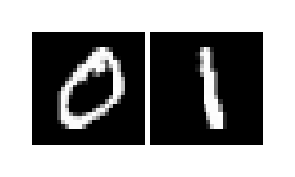
\includegraphics[width=0.08\textwidth]{PaperC/figures/mcts_tikz/dataset_two_images/dataset1.eps}};
    \node[squarednode] (v1) at (9,-1) {\large $\emptyset$};
    
    %%% Task 2 level
    \draw[draw=red!50, fill=red!10, very thick, rounded corners] (0,-2) rectangle (16,-4);
    
    \node[squarednode] (dataset2) at (1.,-3) { \textbf{Task 2} \\ 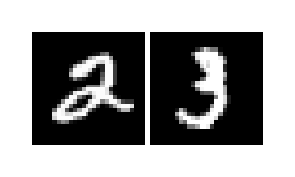
\includegraphics[width=0.08\textwidth]{PaperC/figures/mcts_tikz/dataset_two_images/dataset2.eps}};
    \node[squarednode, text=color3] (v2) at (9,-3) {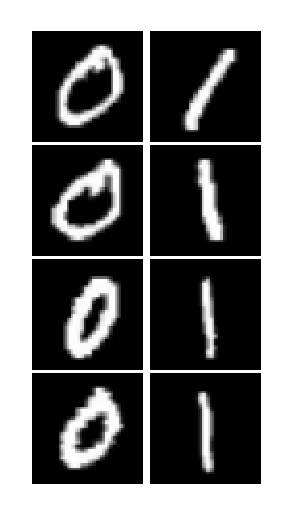
\includegraphics[width=0.045\textwidth]{PaperC/figures/mcts_tikz/vertical_rs/task1_only.eps}};
    \draw[<-] (v2) -- (v1);
    
    %%% Task 3 level
    \draw[draw=color3!50, fill=color3!10, very thick, rounded corners] (0,-4) rectangle (16,-6);
    \node[squarednode] (dataset3) at (1.,-5) { \textbf{Task 3} \\ 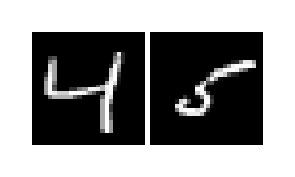
\includegraphics[width=0.08\textwidth]{PaperC/figures/mcts_tikz/dataset_two_images/dataset3.eps}};
    \node[squarednode, text=color3] (v3_beg) at (5,-5) {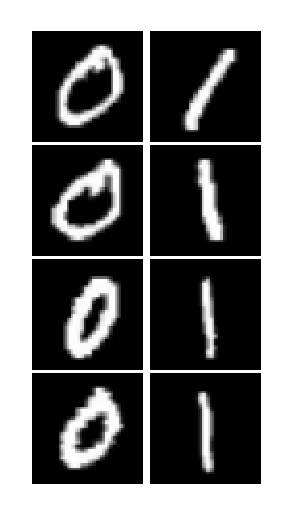
\includegraphics[width=0.045\textwidth]{PaperC/figures/mcts_tikz/vertical_rs/task1_only.eps}};
    \draw[<-, blue, very thick] (v3_beg) -- (v2);
    
    \node[squarednode, text=color3] (v3_mid) at (9,-5) {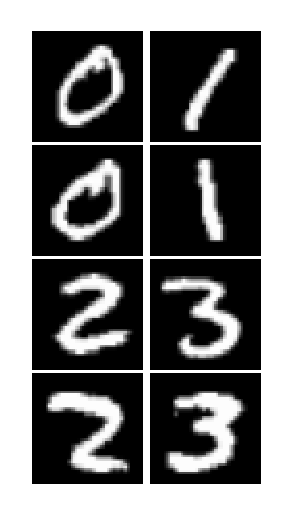
\includegraphics[width=0.045\textwidth]{PaperC/figures/mcts_tikz/vertical_rs/equal_task3.eps}};
    \draw[<-, red, very thick] (v3_mid) -- (v2);
    
    \node[squarednode, text=color3] (v3_end) at (13,-5) {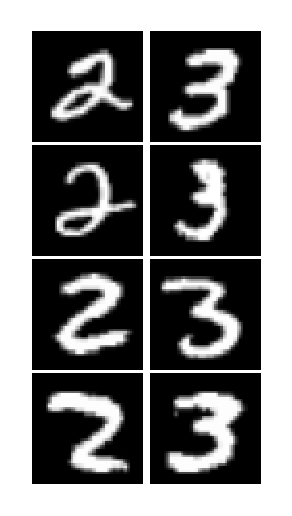
\includegraphics[width=0.045\textwidth]{PaperC/figures/mcts_tikz/vertical_rs/task2_only.eps}};
    \draw[<-, purple, very thick] (v3_end) -- (v2);
    
    %%% Task 4 level
    \draw[draw=magenta!50, fill=magenta!10, very thick, rounded corners] (0,-6) rectangle (16,-8);
    
    \node[squarednode] (dataset4) at (1.,-7) { \textbf{Task 4} \\ 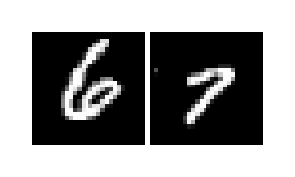
\includegraphics[width=0.08\textwidth]{PaperC/figures/mcts_tikz/dataset_two_images/dataset4.eps}};
    
    \node[squarednode, text=color3] (v41_beg) at (4,-7) {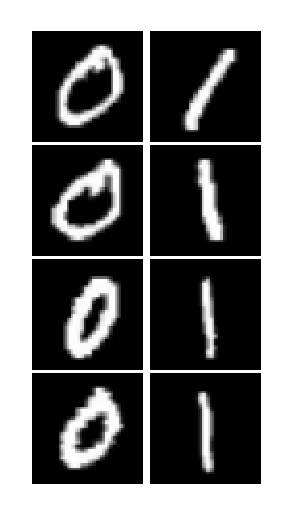
\includegraphics[width=0.045\textwidth]{PaperC/figures/mcts_tikz/vertical_rs/task1_only.eps}};
    \draw[<-, blue, very thick] (v41_beg) -- (v3_beg);
    %\draw[<-] (v4_beg) -- (v3_mid);
    %\draw[<-] (v4_beg) -- (v3_end);
    
    \node[] (v41_dots) at (5,-7) {\large $\cdots$};
    %\draw[<-] (v4_dots1) -- (v3_beg);%\draw[<-, dashed] (v4_dots1) -- (v3_beg);
    %\draw[<-] (v4_dots1) -- (v3_mid);
    %\draw[<-] (v4_dots1) -- (v3_end);
    
    \node[squarednode, text=color3] (v41_end) at (6,-7) {\includegraphics[width=0.045\textwidth]{PaperC/figures/mcts_tikz/vertical_rs/task3_only.eps}};
    \draw[<-] (v41_end) -- (v3_beg);
    
    \node[squarednode, text=color3] (v42_beg) at (7.1,-7) {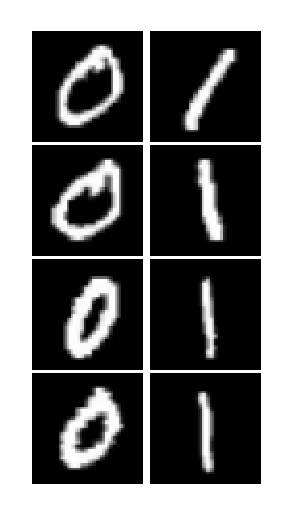
\includegraphics[width=0.045\textwidth]{PaperC/figures/mcts_tikz/vertical_rs/task1_only.eps}};
    \draw[<-] (v42_beg) -- (v3_mid);
    
    \node[] (v42_dots1) at (8,-7) {\large $\cdots$};
    
    \node[squarednode, text=color3] (v42_mid) at (9,-7) {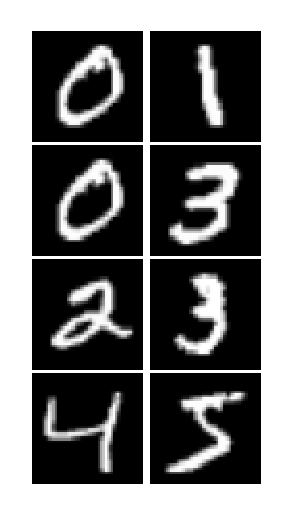
\includegraphics[width=0.045\textwidth]{PaperC/figures/mcts_tikz/vertical_rs/equal_task4.eps}};
    \draw[<-, red, very thick] (v42_mid) -- (v3_mid);
    
    \node[] (v42_dots2) at (10,-7) {\large $\cdots$};
    
    \node[squarednode, text=color3] (v42_end) at (11,-7) {\includegraphics[width=0.045\textwidth]{PaperC/figures/mcts_tikz/vertical_rs/task3_only.eps}};
    \draw[<-] (v42_end) -- (v3_mid);
    %\node[squarednode, text=color3] (v4_end1) at (6.5,-7) {\includegraphics[width=0.08\textwidth]{PaperC/figures/mcts_tikz/replay_batches/task3_only.eps}};
    %\draw[<-] (v4_end1) -- (v3_beg);
    
    \node[squarednode, text=color3] (v43_beg) at (12.1,-7) {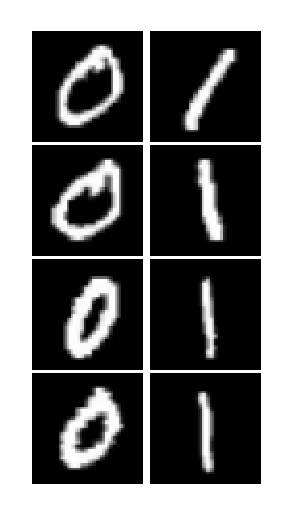
\includegraphics[width=0.045\textwidth]{PaperC/figures/mcts_tikz/vertical_rs/task1_only.eps}};
    \draw[<-] (v43_beg) -- (v3_end);
    
    \node[] (v43_dots) at (13,-7) {\large $\cdots$};
    %\draw[<-] (v4_dots2) -- (v3_beg);
    %\draw[<-] (v4_dots2) -- (v3_mid);
    %\draw[<-] (v4_dots2) -- (v3_end);
    
    \node[squarednode, text=color3] (v43_end) at (14,-7) {\includegraphics[width=0.045\textwidth]{PaperC/figures/mcts_tikz/vertical_rs/task3_only.eps}};
    \draw[<-, purple, very thick] (v43_end) -- (v3_end);
    %\draw[<-] (v4_end) -- (v3_mid);
    %\draw[<-, purple, very thick] (v4_end) -- (v3_end);


    %%% Task 5 level
    \draw[draw=green!50, fill=green!10, very thick, rounded corners] (0,-8) rectangle (16,-10);
    \node[squarednode] (dataset5) at (1.,-9) { \textbf{Task 5} \\ 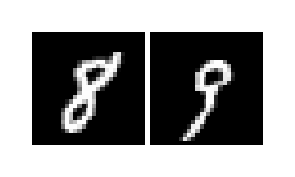
\includegraphics[width=0.08\textwidth]{PaperC/figures/mcts_tikz/dataset_two_images/dataset5.eps}};
    
    \node[squarednode, text=color3] (v51_beg) at (3,-9) {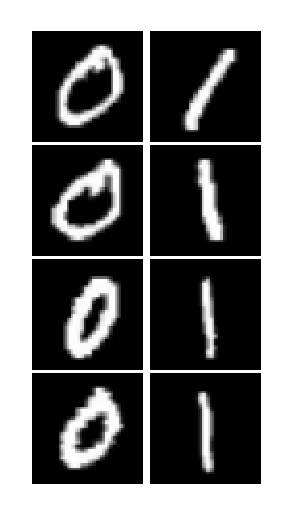
\includegraphics[width=0.045\textwidth]{PaperC/figures/mcts_tikz/vertical_rs/task1_only.eps}};
    \draw[<-, blue, very thick] (v51_beg) -- (v41_beg);
    %\draw[<-] (v5_beg) -- (v4_dots1);
    %\draw[<-] (v5_beg) -- (v4_mid);
    %\draw[<-] (v5_beg) -- (v4_dots2);
    %\draw[<-] (v5_beg) -- (v4_end);
    
    \node[] (v51_dots) at (4,-9) {\large $\cdots$};
    %\draw[<-] (v5_dots1) -- (v4_beg1);
    %\draw[<-] (v5_dots1) -- (v4_dots1);
    %\draw[<-] (v5_dots1) -- (v4_mid);
    %\draw[<-] (v5_dots1) -- (v4_dots2);
    %\draw[<-] (v5_dots1) -- (v4_end);
    
    \node[squarednode, text=color3] (v51_end) at (5,-9) {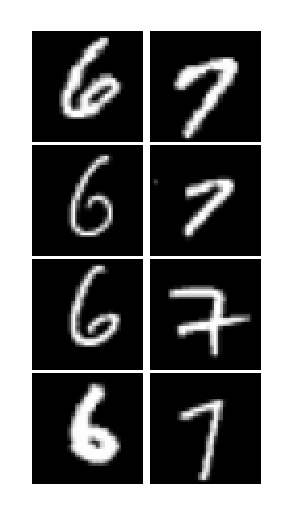
\includegraphics[width=0.045\textwidth]{PaperC/figures/mcts_tikz/vertical_rs/task4_only.eps}};
    \draw[<-] (v51_end) -- (v41_beg);
    
    %\node[squarednode, text=color3] (v52_beg) at (5,-9) {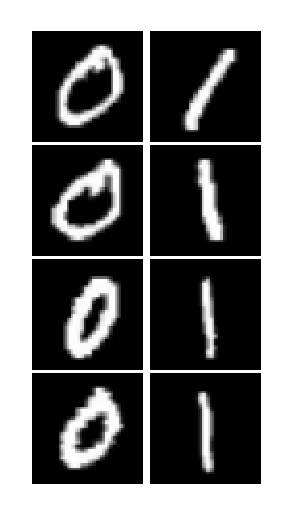
\includegraphics[width=0.045\textwidth]{PaperC/figures/mcts_tikz/vertical_rs/task1_only.eps}};
    
    %\node[squarednode, text=color3] (v5_mid_low) at (6,-9) {\includegraphics[width=0.06\textwidth]{PaperC/figures/mcts_tikz/replay_batches/task5_middle0.eps}};
    %\draw[<-] (v5_mid_low) -- (v4_beg);
    %\draw[<-] (v5_mid_low) -- (v4_dots1);
    %\draw[<-] (v5_mid_low) -- (v4_mid);
    %\draw[<-] (v5_mid_low) -- (v4_dots2);
    %\draw[<-] (v5_mid_low) -- (v4_end);
    
    \node[] (v52_dots) at (6,-9) {\large $\cdots$};
    \draw[<-, dashed] (v52_dots) -- (v41_end);
    
    \node[] (v53_dots) at (7.1,-9) {\large $\cdots$};
    \draw[<-, dashed] (v53_dots) -- (v42_beg);
    
     \node[] (v54_dots) at (8,-9) {\large $\cdots$};
    %\draw[<-] (v5_dots2) -- (v4_beg);
    %\draw[<-] (v5_dots2) -- (v4_dots1);
    %\draw[<-] (v5_dots2) -- (v4_mid);
    %\draw[<-] (v5_dots2) -- (v4_dots2);
    %\draw[<-] (v5_dots2) -- (v4_end);
    
    \node[squarednode, text=color3] (v52_mid) at (9,-9) {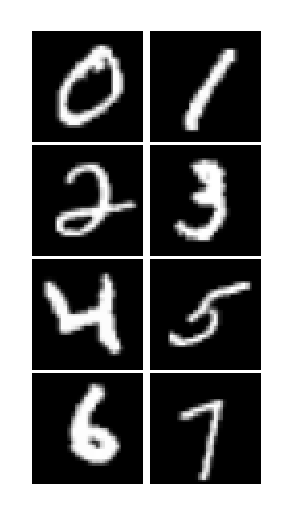
\includegraphics[width=0.045\textwidth]{PaperC/figures/mcts_tikz/vertical_rs/equal_task5.eps}};
    \draw[<-, red, very thick] (v52_mid) -- (v42_mid);
    %\draw[<-] (v5_mid) -- (v4_beg);
    %\draw[<-] (v5_mid) -- (v4_dots1);
    %\draw[<-, red, very thick] (v5_mid) -- (v4_mid);
    %\draw[<-] (v5_mid) -- (v4_dots2);
    %\draw[<-] (v5_mid) -- (v4_end);
    
    \node[] (v55_dots) at (10,-9) {\large $\cdots$};
    
    \node[] (v56_dots) at (11,-9) {\large $\cdots$};
    \draw[<-, dashed] (v56_dots) -- (v42_end);
    
    \node[] (v57_dots) at (12.1,-9) {\large $\cdots$};
    \draw[<-, dashed] (v57_dots) -- (v43_beg);
    %\draw[<-] (v5_dots3) -- (v4_beg);
    %\draw[<-] (v5_dots3) -- (v4_dots1);
    %\draw[<-] (v5_dots3) -- (v4_mid);
    %\draw[<-] (v5_dots3) -- (v4_dots2);
    %\draw[<-] (v5_dots3) -- (v4_end);
    
    %\node[squarednode, text=color3] (v5_mid_high) at (12,-9) {\includegraphics[width=0.06\textwidth]{PaperC/figures/mcts_tikz/replay_batches/task5_middle1.eps}};
    %\draw[<-] (v5_mid_high) -- (v4_beg);
    %\draw[<-] (v5_mid_high) -- (v4_dots1);
    %\draw[<-] (v5_mid_high) -- (v4_mid);
    %\draw[<-] (v5_mid_high) -- (v4_dots2);
    %\draw[<-] (v5_mid_high) -- (v4_end);
    
    \node[squarednode, text=color3] (v53_beg) at (13,-9) {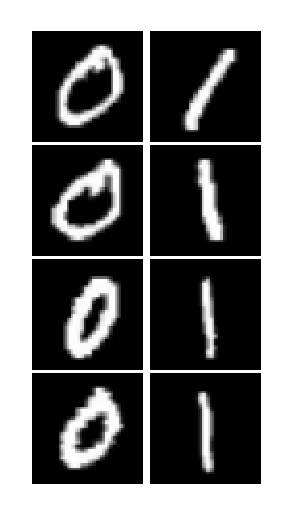
\includegraphics[width=0.045\textwidth]{PaperC/figures/mcts_tikz/vertical_rs/task1_only.eps}};
    \draw[<-] (v53_beg) -- (v43_end);
    
    \node[black] (v58_dots) at (14,-9) {\large $\cdots$};
    
    %\draw[--, dashed] (v5_dots4) -- (v43_dots);
    %\draw[<-] (v5_dots4) -- (v4_mid);
    %\draw[<-] (v5_dots4) -- (v4_dots2);
    %\draw[<-] (v5_dots4) -- (v4_end);
    
    \node[squarednode, text=color3] (v53_end) at (15,-9) {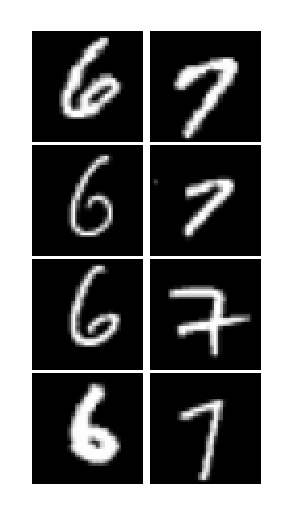
\includegraphics[width=0.045\textwidth]{PaperC/figures/mcts_tikz/vertical_rs/task4_only.eps}};
    \draw[<-, purple, very thick] (v53_end) -- (v43_end);
    %\draw[<-] (v5_end) -- (v4_beg);
    %\draw[<-] (v5_end) -- (v4_dots1);
    %\draw[<-] (v5_end) -- (v4_mid);
    %\draw[<-] (v5_end) -- (v4_dots2);
    %\draw[<-, purple, very thick] (v5_end) -- (v4_end);
\end{tikzpicture}
}
  % \tikzexternalenable
  % \vspace{-15pt}
  % \includegraphics[width=0.95\linewidth]{pixeldag.png}
  % \vspace{-15pt}
